\chapterimage{band1.png}
\chapter{Variáveis}\label{cap:memoria}
Tal como nós, as pessoas, utilizamos o cérebro para memorizar informação para utilizar mais tarde, também um computador necessita de armazenar temporariamente dados para trabalhar.

Este capítulo descreve como os nossos programas podem armazenar dados e manipulá-los.

\section{Memória e Variáveis}
A memória%
\footnote{A memória utilizada pelos programas é a famosa memória RAM (\emph{Random Access Memory}) que aparece nas especificações técnicas dos computadores.}
 é o que permite ao nosso programa guardar dados temporários ou intermédios para serem utilizados mais tarde.
Por exemplo%
\footnote{O exemplo é uma adaptação do Exemplo~\ref{exe:calcularpontuacaoFCP} do primeiro capítulo.}%
, se pretendessemos criar um programa para calcular os pontos da equipa do FCP no campeonato fariamos algo do género:
\begin{lstlisting}[caption=Pontos do FCP (sintaxe Processing), label=exe:pontosFCPProcessing]
int jogosGanhos;
int jogosEmpatados;
int pontos;

jogosGanhos = 5;
jogosEmpatados = 2;

pontos = jogosGanhos * 3 + jogosEmpatados;

print(pontos);
\end{lstlisting}
No programa anterior a instrução \texttt{jogosGanhos = 5} (não nos vamos preocupar, para já, com as primeiras três linhas), coloca numa \emph{variável} (na memória) o valor 5. Uma variável
é a memória do nosso programa. É como uma gaveta com nome, na qual podemos guardar valores para mais tarde utilizar.
O programa anterior precisa de guardar os valores do número de jogos ganhos e empatados para poder efectuar a operação matemática que devolve o número de pontos no campeonato. O resultado desse cálculo, é, ele mesmo, colocado também numa ``gaveta'' para posterior utilização. Uma vez colocados na ``gaveta'' (variável), os dados podem ser consultados em qualquer altura (ponto de execução) do nosso programa. 

As variáveis têm de ter um nome. O nome é o identificador utilizado no programa e que representa uma posição na memória do computador. Os nomes das variáveis são palavras com uma ou mais letras, dígitos e ``\_'' (\emph{underscore}). Os nomes
não podem começar por um dígito. Para facilitar a leitura do código, utiliza-se frequentemente a notação ``camelo'',
i.e., os nomes das variáveis começam por uma palavra em letra minúscula seguido de uma ou mais palavras cuja primeira
letra é maiúscula. Por exemplo: \texttt{nomeDaVariavel}.

Para além do nome, as variáveis têm de ter um \emph{tipo}. No exemplo anterior, as primeiras três linhas definem os tipos das variáveis. 

\section{Guerra dos Tipos (Tipos de Dados)}
Os dados armazenados e manipulados pelo programa têm determinadas características que fazem
com que seja possível realizar determinadas operações sobre esses dados. Por exemplo, não
faz sentido somar a palavra ``jorge'' com o valor numérico $20$; mas faz sentido somar $10$ com $10$. As
operações apenas fazem sentido se os dados sobre os quais operam forem compatíveis%
\footnote{Compatível não significa necessariamente do mesmo tipo; podemos somar, por exemplo, um número inteiro com um número fraccionário. }%
.

De uma forma geral, podemos trabalhar com dois tipos de dados simples: valores numéricos (que podem ser divididos em 
valores inteiros e valores reais) e valores lógicos (verdadeiro ou falso). Existem também dados complexos como texto. Podemos também agrupar
dados simples em estruturas mais complexas como vectores e matrizes.

\begin{description}
\item[Inteiro]
O tipo \emph{Inteiro} permite armazenar valores numéricos inteiros, i.e., sem casas decimais. 

\item[Real]
O tipo \emph{Real} armazena valores numéricos reais, i.e., números com casas decimais.

\item[Lógico]
O tipo \emph{Lógico} armazena apenas os valores \emph{verdadeiro} ou \emph{falso}.

\item[Texto]
O tipo \emph{Texto} armazena dados na forma de texto, e.g., ``O nome é:''.

\item[Vector]
O tipo \emph{Vector}%
\footnote{Vector não é propriamente um tipo de dados, mas antes uma estrutura de agrupamento de dados, uma vez que os vectores podem ser de vários tipos. O mesmo se aplica à Matriz.}
 é um tipo de dados complexo que consiste numa sequência de valores do mesmo tipo. Os
vectores podem ser de qualquer um dos tipos simples, i.e., podemos criar vectores de inteiros, reais, lógicos ou texto.
Usando vectores podemos armazenar vários valores sem ter de os nomear individualmente. Os valores individuais dos vectores
são acedidos através do seu índice.

\item[Matriz]
Uma \emph{Matriz} é uma generalização do vector para várias dimensões.
\end{description}

Este capítulo irá abordar apenas os tipos de dados simples. Os dados complexos serão abordados mais à frente.

Em Processing, os tipos simples descritos anteriormente são representados pelas seguintes \emph{keywords}%
\footnote{\emph{keyword} -- palavra chave -- são palavras reservadas pela linguagem de programação para a sua sintaxe. Isto significa que as \emph{keywords} têm um significado especial para a linguagem pelo que não podem ser usadas como nomes de variáveis (nem como nomes de métodos).}%
:
\begin{center}
\begin{tabular}{ll}
Tipo de variável 	& \emph{Keyword} do Processing\\
\hline
Inteiro 					& \texttt{int}\\
Real							& \texttt{float}\\
Lógico						& \texttt{boolean}\\
\hline
\end{tabular}
\end{center}
Estes são os tipos mais utilizados, mas existem muitos outros. A Tabela~\ref{tab:tiposprimitivos} lista os tipos primitivos e o tamanho que ocupam em memória.

\begin{table}[!hb]
\centering
{\small
\begin{tabular}{lll}
\emph{Keyword}					&Descrição																			& Tamanho/Gama \\
\hline
(Números Inteiros)			&&\\
\texttt{byte}						&Byte																						&8-bit\\
												& 																							&(-128 a 127)\\
\texttt{short}					&Inteiro curto																	&16-bit\\
												& 																							&(-32768 a 32767)\\
\emph{\texttt{int}}			&Inteiro																				&32-bit\\
												&																								&(-2147483648 a 2147483647)\\
\texttt{long}						&Inteiro longo																	&64-bit\\
												&																								&(-9223372036854775808 a ...807)\\
\hline
(Números Reais)					&&\\
\emph{\texttt{float}}		& Vírgula flutuante 														&32-bit IEEE 754\\
												&de precisão simples														&(1.40129846432481707e-45 a\\ 
												&																								&3.40282346638528860e+38) (positivo ou negativo)\\
\texttt{double}					& Vírgula flutuante 														&	64-bit IEEE 754\\
												& de dupla precisão															&(4.94065645841246544e-324 a\\
												&  																							& 1.79769313486231570e+308) (positivo ou negativo)	\\
\hline
(Outros)								&&\\
\texttt{char} 					&	Um carácter																		&16-bit Unicode\\
\emph{\texttt{boolean}}	& Valor lógico 																	&1-bit\\
& (\emph{true} ou \emph{false})		& \\
\end{tabular}}
\caption{Tabela de tipos primitivos do Processing}\label{tab:tiposprimitivos}
\end{table}
%\subsubsection{Tipos Complexos}
%\begin{tabular}{lll}
%\emph{Keyword}					&Descrição																			& Tamanho/Gama\\
% \hline
%\texttt{String} 				&String (cadeia de caracteres) -- Texto					& \\
%\texttt{array}					& Vector																				& \\
%\end{tabular}
\section{Declaração de Variáveis}
A \emph{declaração} de uma variável é feita indicando o \emph{tipo} da variável seguido do seu nome. Declarar uma variável é indicar que o nosso programa irá precisar de um bocado de memória do computador para guardar dados. Desta forma o Processing pode reservar esse pedaço de memória%
\footnote{No caso de variáveis de tipos simples, basta declarar para reservar espaço em memória. No caso de variáveis de tipos complexos é preciso fazer algo mais. Isto será descrito nos capítulos mais à frente.}%
.

Em Processing, \textbf{todas} as variáveis têm de ser declaradas antes de poderem ser utilizadas pelo programa.

No programa do Exemplo~\ref{exe:pontosFCPProcessing}, as três primeiras linhas correspondem à declaração das variáveis utilizadas pelo nosso programa%
\footnote{Neste exemplo, as três variáveis foram declaradas em três linhas diferentes por uma questão de legibilidade do programa. No entanto, como são todas do mesmo tipo poderiam ter sido declaradas na mesma linha: \texttt{int jogosGanhos, jogosEmpatados, pontos;}.}%
.

Os exemplo seguinte mostra um programa simples em Processing com declaração de variáveis.

\begin{minipage}{\textwidth}
\begin{center}
	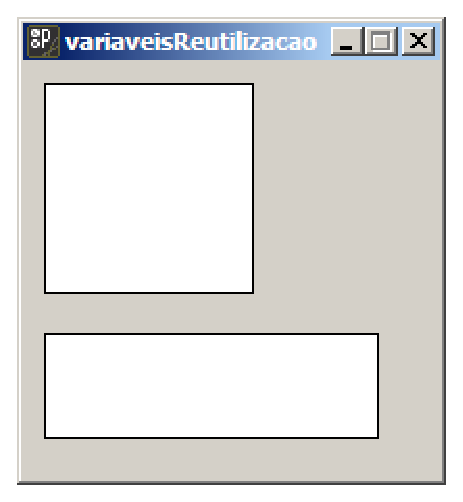
\includegraphics[width=4cm]{images/variaveisReutilizacao.eps}
\end{center}
\begin{lstlisting}[caption=Reutilização de variáveis, label=exe:variaveisReutilizacao]
int larguraRectangulo;
int alturaRectangulo;

size(200, 200); //define a largura da janela: 200x200

larguraRectangulo = 100; // largura 100 para o primeiro rectangulo.
alturaRectangulo = 100;  // altura 100 para o primeiro rectangulo.
rect(10, 10, larguraRectangulo, alturaRectangulo); // desenha o rectangulo na posicao 10, 10.

larguraRectangulo = 160; // largura 160 para o segundo rectangulo.
alturaRectangulo = 50;   // altura 50 para o segundo rectangulo.
rect(10, 130, larguraRectangulo, alturaRectangulo); // desenha o rectangulo na posicao 10, 130.
\end{lstlisting}
\end{minipage}

No programa do exemplo anterior podemos ver que as variáveis declaradas são utilizadas várias vezes no nosso programa.


\section{Guardar na Gaveta (Atribuição)}
As variáveis apenas têm utilidade se lhes podermos alterar e ler o seu conteúdo. Para colocarmos um valor%
\footnote{Colocar um valor numa variável é \emph{atribuir} um valor a essa variável.}
 numa variável basta escrever numa linha o nome da variável seguido do símbolo ``='' (igual), seguido do valor que pretendemos atribuir e terminando com ``;'' (ponto e vírgula).
Ou seja, algo do género (os programas anteriores já tinham instruções destas)%
\footnote{Neste programa, faço uma atribuição de um valor decimal a uma variável. Em Processing, as casas decimais são separadas por um ``.'' (ponto) e não por ``,'' (vírgula).}%
:
\begin{lstlisting}
float minhaVariavel; //primeiro temos sempre de declarar a variável.

minhaVariavel = 102.4; //atribuir o valor 102.4
\end{lstlisting}


Uma variável guarda sempre um valor durante o programa, mas esse valor pode ser alterado em qualquer ponto do programa pela atribuição, pelo que podemos fazer com que uma variável guarde valores diferentes em momentos diferentes do programa:
\begin{lstlisting}
int x;
int y;

x = 0;
y = 0;
point(x, y);

x = 2;
y = 3;
point(x, y);
\end{lstlisting}
Este programa utiliza a mesma instrução duas vezes -- \texttt{point(x, y)} -- mas em momentos diferentes no programa, pelo que o resultado da execução das duas instruções é diferente.
Na primeira, \texttt{point(x, y)} da linha 6, pode ser substituida por \texttt{point(0, 0)} (\texttt{x} e \texttt{y} têm ambas o valor zero, neste ponto).
Na segunda, \texttt{point(x, y)} da linha 10, pode ser substituida por \texttt{point(2, 3)} (neste ponto \texttt{x} tem o valor 2 e \texttt{y} tem o valor 2). 
O resultado deste programa seria o desenho de dois pontos (pixeis) no ecrã: um na posição (0, 0) e outro na posição (2, 3).


\subsection{Inicialização}
Um conceito associado com a declaração de variáveis é a \emph{inicialização} de variáveis. Antes de podermos utilizar o valor de uma variável, é necessário que essa variável contenha algum valor. Caso contrário, qual seria o resultado? Observem o programa seguinte:
\begin{lstlisting}
int x;
int y;

point(x, y);
\end{lstlisting}
Em que posição do ecrã irá ser desenhado o ponto?

Se responderam (0, 0), estão errados :).

O valor zero (0) parece o mais óbvio, mas de facto, em Processing%
\footnote{Em algumas linguagens de programação, é, de facto, o zero! Nessas linguagens as variáveis são inicializadas automaticamente com o valor zero, se o programador não as inicializar.}%
, não é assim. Se experimentarem correr este programa no Processing irão deparar-se com um erro de compilação. Em Processing, não é possível utilizar uma variável que não tenha sido inicializada, ou seja, uma variável à qual ainda não tenha sido feita uma atribuição.

Para corrigir o programa anterior teriamos então de inicializar as duas variáveis:
\begin{lstlisting}
int x;
int y;

x = 0;
y = 4;
point(x, y);
\end{lstlisting}
Reparem que não é necessário inicializar uma variável com o valor zero. Podemos inicializa-las com qualquer valor que faça sentido no nosso programa!

\subsection{Combinar Declaração com Atribuição}
Uma vez que, depois de declarar uma variável, é obrigatório inicializá-la, o Processing fornece-nos uma forma de fazer estes dois passos mais rapidamente: combinando a declaração com a inicialização. 
O exemplo seguinte mostra como se faz isto:
\begin{lstlisting}
int x = 0;
int y = 4;

point(x, y);
\end{lstlisting}

\section{Visibilidade}
É possível fazer a declaração de variáveis em qualquer ponto do programa, embora seja boa prática fazê-lo no início do programa.
É possível mesmo declarar variáveis dentro de métodos%
\footnote{Vamos ver num capítulo mais à frente exactamente o que são métodos. Para já, podemos considerá-los como pedaços de código com nome, ou seja, blocos de código que podem ser chamados (executados) pelo nome.}%
:
\begin{lstlisting}
int x; //variável global
int y; //variável global

void setup() {
    int z = 4; //variável local ao setup()
	  
    size(200, 200);
    x = 0;
    y = 0;
}

void draw() {	
    point(x, y);
}
\end{lstlisting}
O exemplo anterior, utiliza três variáveis: \texttt{x}, \texttt{y} e \texttt{z}. As primeiras duas estão declaradas no início do programa. A variável \texttt{z} está declarada dentro do método \texttt{setup()}.

Dizemos que as variáveis \texttt{x} e \texttt{y} são variáveis globais e a variável \texttt{z} é uma variável local.
As variáveis globais são variáveis que são visíveis, isto é, podem ser utilizadas, em qualquer ponto do programa. No caso do exemplo, as variáveis \texttt{x} e \texttt{y}, apesar de declaradas fora do \texttt{draw()}, são utilizadas lá dentro.

As variáveis locais apenas podem ser utilizadas dentro do bloco onde foram declaradas: a variável \texttt{z} foi declarada dentro do bloco correspondente ao método \texttt{setup()} pelo que apenas pode ser utilizada dentro desse método.
Se tentássemos utilizá-la noutro sítio, como por exemplo:
\begin{lstlisting}
int x; //variável global
int y; //variável global

void setup() {
    int z = 4; //variável local ao setup()	  
    size(200, 200);
    x = 0;
    y = 0;
}

void draw() {	
    point(x, y);
	
    point(z, 5); //erro! 'z' só é conhecida dentro de setup() e nao draw()
}
\end{lstlisting}
Este programa não iria compilar: a variável \texttt{z} utilizada em \texttt{draw()} não é conhecida.

Então porque não utilizar sempre variáveis globais? 

As variáveis globais consomem memória (afinal, as variáveis \textbf{são} memória) do computador durante toda a execução do programa. As variáveis locais apenas consomem memória enquanto o bloco está a executar. Para além disso, no caso de programas muito complexos, tornar-se-ia confuso para o programador ter uma lista muito grande de variáveis globais, quando algumas apenas são utilizadas dentro de um método!

Assim, se apenas precisarmos de uma variável para contas intermédias dentro de um método, devemos declarar essa variável local a esse método.

%--------------
O lugar onde declaramos as variáveis no nosso programa: corpo principal ou dentro dos métodos, pode ser visto como uma estrutura de caixas dentro de caixas. 
%--------------
\section{Instruções}
Já vimos, até aqui, que podemos atribuir valores a variáveis. No entanto, as instruções de atribuição que vimos até agora foram todas muito básicas. 

O valor que atribuimos a uma variável pode ser uma valor literal ou o resultado da avaliação de uma expressão com variáveis, métodos, etc.
\emph{Literal}, em programação, é um valor codificado directamente na instrução. Por exemplo, na instrução
\begin{lstlisting}
x = 10;
\end{lstlisting}
o valor 10 é um literal. 

\subsection{Operadores Aritméticos} 
Soma (+); subtracção (-); multiplicação (*); divisão(/); resto da divisão (\%). Os operadores aritméticos podem ser usados sobre dados do tipo inteiro ou real. 

Os operadores aritméticos podem ser combinados:
\begin{lstlisting}
int x = 2;
int y;
y = 2 + x * 4;
\end{lstlisting}

É preciso ter cuidado, no entanto, com a ordem com que as operações são efectuadas. No caso do exemplo anterior que operação é efectuada primeiro? $2 + x$, ou $x * 4$?
Para resolver este problema existe a noção de precedência das operações. No caso das operações aritméticas, a multiplicação,
divisão e resto da divisão têm maior precedência do que a soma e subtracção, o que significa que são efectuadas primeiro. 
Se a precedência das operações for igual, então as operações são feitas da esquerda para a direita (associatividade à esquerda).

Se quisermos que determinada operação tenha precedência sobre outra podemos utilizar os parêntesis:
\begin{lstlisting}
int y;

y = 2 / (x + 4);
\end{lstlisting}
Neste caso, a soma irá ser efectuada antes da divisão.

Quando temos expressões muito complexas, é boa prática utilizar os parêntesis, mesmo que o problema da precedência
não se coloque. A utilização de parêntesis facilita a leitura da expressão.

\subsection{Uma Operação Complicada! (Instruções Complexas)}

Para além das expressões matemáticas podemos também utilizar nas instruções chamadas a métodos%
\footnote{Em programação existem dois tipos de métodos: métodos que devolvem um valor e métodos que não devolvem valor nenhum. Nas expressões de atribuição podemos utilizar métodos que retornam valores.}%
:
\begin{lstlisting}
int x = 0;
int y = 6;

x = y * 5 + sqrt(16);
\end{lstlisting}
O método \texttt{sqrt(16)} devolve o valor da raiz quadrada de 16. Quando o programa chegar à expressão de atribuição irá substituir automaticamente os valores das variáveis e métodos pelos seus valores actuais. Ou seja, a expressão \texttt{y * 5 + sqrt(16)} é o mesmo que \texttt{6 * 5 + 4} que será igual a \texttt{34}.

Este processo de substituição pode ser utilizar em qualquer nível de profundidade:
\begin{lstlisting}
int x = 0;
int y = 6;

x = y * 5 + sqrt(y*6+sqrt(169);
\end{lstlisting}
A expressão \texttt{y * 5 + sqrt(y*6+sqrt(169)} será substituída recursivamente por \texttt{6 * 5 + sqrt(6*6+13)} e depois 
por \texttt{30 + sqrt(49)}, depois por \texttt{30 + 7} e finalmente por \texttt{37}.

\section{Exercícios}
\begin{enumerate}
\item \label{exe:3_tipos}
* Indique qual o melhor tipo de variável para cada uma das seguintes situações:
\begin{enumerate}
\item A idade de uma pessoa.
\item O preço de um artigo de supermercado.
\item A nota final de um aluno à cadeira de Programação Multimédia.
\item Armazenar uma pergunta de um teste.
\item O peso de todos os elementos de uma corporação de bombeiros.
\item A cor de cada pixel de uma imagem digital.
\item As alíneas deste conjunto de problemas.
\item O número do BI.
\item Os números de telefone dos seus contactos do telemóvel.
\item Os preços de um determinado artigo de supermercado ao longo dos 12 meses do ano.
\item A sua média de entrada na faculdade.
\end{enumerate}

\item \label{exe:3_declaracao}
* Escreva as instruções de declaração das variáveis da secção anterior.

\item \label{exe:3_1}
* Crie um programa em Processing que desenhe 5 linhas em posições diferentes alterando apenas os valores de variáveis. Ou seja a instrução para desenhar deve ser sempre \texttt{line(x0, y0, x1, y1);}. Altere apenas os valores das variáveis.

\item  \label{exe:3_2} \label{ps:linhaAnimada}
* Crie um programa que anime uma linha no ecrã. Irá ter de utilizar o método \texttt{draw()} (veja um dos exemplos e altere).
Pense nas variáveis que terá de utilizar, onde as deverá inicializar e onde as deverá actualizar. Não faz mal se a sua linha desaparecer do ecrã a certa altura, mas pense no que teria de fazer para evitar isso.

\item  \label{exe:3_3}
* Diga o que está mal no programa seguinte:
\begin{lstlisting}
int largura;

void setup() {
    size(200, 200);
    
    largura = 100;
    altura = 100;
}

void draw() {
    rect(10, 10, largura, altura);
}
\end{lstlisting}
Corrija-o.
\end{enumerate}